\chapter{Literature Review and Related Work}
\label{chap:relatedworks}

\section{Competitor Analysis}
\label{section:competitor-analysis}

The competitive landscape for fitness technology is currently divided between manual tracking applications and high-cost industrial hardware. Prometheus positions itself as an automated, non-intrusive solution that leverages existing infrastructure to provide high-utility data at a lower entry cost for facility owners.

\begin{figure}[h]
    \centering
    % Note: Replace 'example-image' with your actual file name
    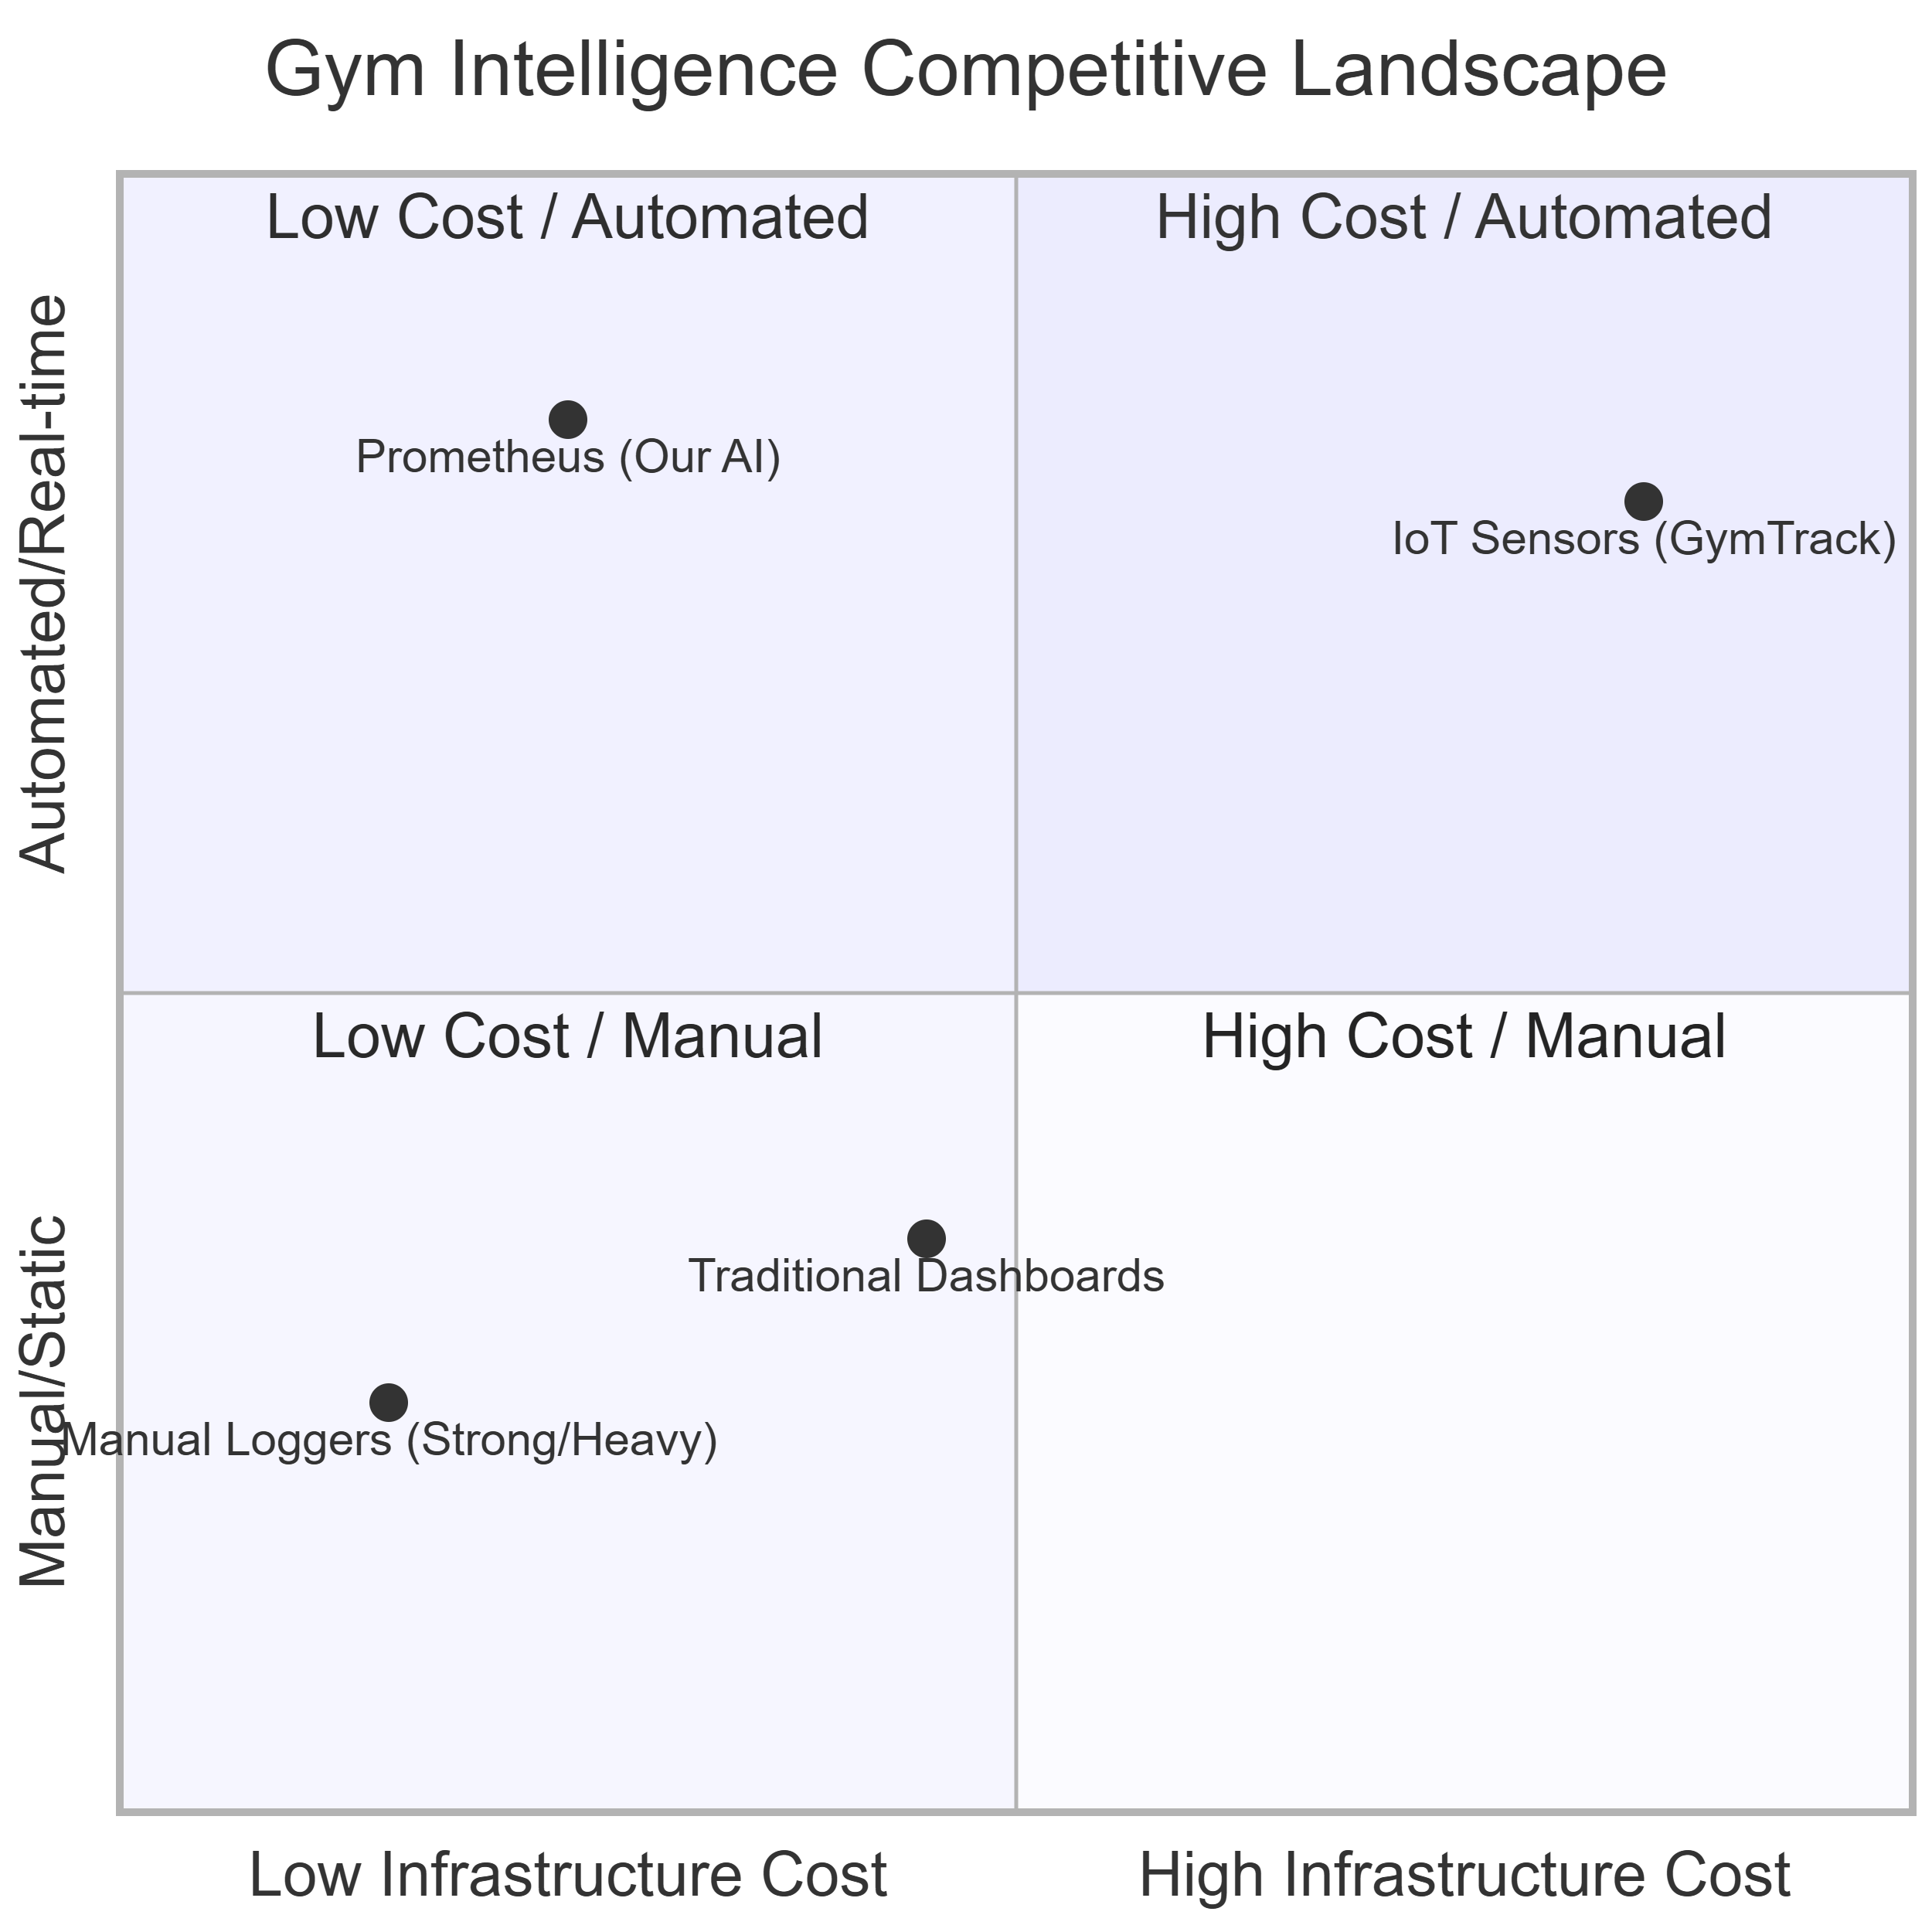
\includegraphics[width=0.8\textwidth]{assets/figures/Competitor.png}
    \caption{Competitive Landscape: Automation vs. Infrastructure Cost}
    \label{fig:competitor-landscape}
\end{figure}

The following table provides a detailed comparison between Prometheus and existing solutions in the market, highlighting the gaps in real-time spatial intelligence.

\begin{table}[h]
\centering
\footnotesize % Reduces font size (can also use \small or \scriptsize)
\renewcommand{\arraystretch}{1.5} % Increases row height for better readability
\setlength{\tabcolsep}{4pt} % Reduces horizontal padding between columns

\begin{tabularx}{\textwidth}{|l|X|X|X|X|}
\hline
\textbf{Feature} & \textbf{Prometheus} & \textbf{Manual Loggers} & \textbf{IoT Sensors} & \textbf{Gym Dashboards} \\ \hline
Real-time Occupancy & Automated CV on RTSP streams & Manual inspection or self-report & Entry/exit counts only & Manual check-in required \\ \hline
Installation Cost & Low; reuses CCTV infrastructure & Zero; pen-and-paper logs & High; per-station sensors & Moderate; software and kiosks \\ \hline
Member Utility & High; live heatmap and forecasts & High for workout logging only & Low; not member-facing & Moderate; schedules only \\ \hline
Spatial Analytics & Full heatmaps and utilisation trends & None & Counts only; no mapping & Check-in data only \\ \hline
Privacy & Edge-only; no raw video shared & High; no video collected & High; no biometric data & Moderate; third-party SaaS \\ \hline
Scalability & Per-camera; add feeds easily & Poor; effort grows linearly & Hardware-limited scaling & Software tier-limited \\ \hline
Maintenance & Periodic retraining; CCTV upkeep & Staff training only & Battery, firmware, hardware failures & Vendor-managed; kiosk servicing \\ \hline
\end{tabularx}
\caption{Comparison Table of Competitive Fitness Solutions}
\label{table:competitor-analysis}
\end{table}

\section{Literature Review}
\label{section:literature-review}

To build a technically sound and feasible system, this project draws from several key academic works and technical advancements in the fields of Computer Vision and Distributed Systems.

\subsection{Real-Time Object Detection (YOLO Architecture)}
The foundation of the occupancy detection engine is based on the ``You Only Look Once'' (YOLO) architecture. Research by Redmon et al. established that frame-rate inference is possible by treating detection as a single regression problem. This project specifically evaluates the use of YOLOv8 and YOLOv10. The selection of YOLOv10 informs our choice for edge deployment, as its elimination of Non-Maximum Suppression (NMS) significantly reduces computational latency on local hardware.

\subsection{Vision-Based Gym Monitoring (GymCam)}
The ``GymCam'' project by Khurana et al. demonstrated the viability of using unconstrained camera feeds to track multiple users and exercises simultaneously. Their research indicates that while fine-grained action recognition is complex, identifying machine occupancy through spatial overlap is highly reliable. Prometheus extends this logic by utilizing a multi-camera RTSP network to provide floor-wide spatial analytics.

\subsection{Large-Scale Multi-View Datasets (M3GYM)}
For model training, this project utilizes the M3GYM dataset. Unlike standard datasets, M3GYM provides multi-view labels in real-world gym environments characterized by high occlusion. This informs the design of our ``Occupancy Logic,'' allowing the system to distinguish between a person walking near equipment and a person actively utilizing a machine.

\subsection{Privacy-Preserving Edge Computing}
A primary constraint for gym-based AI is member privacy (GDPR/PDPA). Current literature suggests that performing inference at the ``edge'' allows raw video data to be discarded immediately after metadata extraction. This informs our choice of an Edge Processing Layer (e.g., ASUS NUC), ensuring that no identifiable video frames are ever transmitted to the cloud.

\subsection{Retail and Commercial Space People Counting}
Vision-based people counting has been extensively deployed in retail environments to measure footfall and dwell time at product shelves. Systems such as those described by Albiol et al. use overhead camera feeds combined with background subtraction and blob tracking to count entrants and exiters at store thresholds. These systems share Prometheus's architectural pattern of fixed-camera inference on a constrained zone, but operate in single-plane entry contexts rather than complex multi-zone floor plans. The retail domain's emphasis on conversion-rate analytics (dwell time versus purchase rate) directly parallels Prometheus's per-equipment utilisation metrics, demonstrating that spatial intelligence derived from CCTV feeds has measurable commercial value beyond security.

\subsection{Smart Building and Office Occupancy Detection}
Occupancy detection for energy management in smart buildings is a well-studied problem. Hailemariam et al. showed that computer-vision-based room occupancy outperforms PIR motion sensors in accuracy because vision captures head-count rather than mere movement. Building Management Systems (BMS) from vendors such as Siemens Enlighted and Cisco Spaces combine ceiling-mounted depth sensors with Wi-Fi probe requests to estimate desk and meeting-room occupancy at scale. Prometheus adopts the same principle of inferring occupancy from non-contact sensing, extending it from single-room granularity to per-equipment granularity across a large open floor plan.

\subsection{Crowd Density Estimation in Public Spaces}
Crowd density estimation research, originating from public safety applications in transportation hubs and stadiums, provides techniques directly applicable to high-density gym floors. Zhang et al.'s CSRNet demonstrated that dilated convolutional networks can generate density maps from heavily occluded scenes without per-person bounding boxes, making inference tractable even when individuals overlap. While Prometheus targets lower crowd densities than stadium scenarios, the density-map paradigm informs our heatmap visualisation layer, where pixel-level density estimates are aggregated into zone-level utilisation scores displayed on the facility dashboard.

\subsection{Sports and Athlete Tracking Systems}
Professional sports analytics systems such as Second Spectrum (NBA/EPL) and Hawk-Eye (tennis, cricket) demonstrate that multi-camera triangulation can yield sub-centimetre positional accuracy for tracking individuals in a bounded arena. At a lower cost tier, research by Gade et al. using overhead thermal cameras in sports halls achieved robust person tracking under varying lighting without privacy concerns, since thermal imagery is non-identifiable. These approaches validate the principle of camera-network-based spatial tracking used by Prometheus, while also establishing the thermal camera as a privacy-safe sensing modality that may be considered for future iterations where GDPR compliance is critical.

\subsection{Hospital and Healthcare Facility Flow Analysis}
Patient flow and staff utilisation tracking in hospitals presents challenges structurally similar to gym equipment monitoring: high asset density, frequent short-duration interactions, and strong privacy requirements. Systems reviewed by Ajami et al. use RFID badges combined with zone antennas to track patient dwell times at care stations. Computer-vision alternatives, explored by Bao et al., replace RFID with overhead camera pose estimation to infer staff activity without wearable hardware. The healthcare domain's regulatory focus on anonymisation (HIPAA/PDPA) aligns with Prometheus's edge-processing privacy model and reinforces the design decision to transmit only aggregated metadata rather than video or biometric identifiers.